\documentclass[a4paper]{article}

\usepackage{amsmath,amssymb,amsfonts}
\usepackage{amssymb, amsmath}
\usepackage{ascmac}
\usepackage{algorithmic}

\DeclareMathOperator{\Bern}{\rm Bern}
\DeclareMathOperator{\Bin}{\rm Bin}
\DeclareMathOperator{\Po}{\rm Po}
\DeclareMathOperator{\Cat}{\rm Cat}
\DeclareMathOperator{\Mult}{\rm Mult}
\DeclareMathOperator{\Beta}{\rm Beta}
\DeclareMathOperator{\Dir}{\rm Dir}
\DeclareMathOperator{\N}{\mathcal{N}}
\DeclareMathOperator{\InvW}{\mathcal{IW}}
\DeclareMathOperator{\NIW}{\mathcal{NIW}}

\newcommand{\proptoas}[1]{\overset{#1}{\propto}}
\DeclareMathOperator{\defeq}{\ensuremath{\stackrel{\mathrm{def}}{=}}}

\usepackage{braket}
\usepackage{url}

\usepackage[dvipdfmx]{graphicx}

\title{Sample of HSMM parameters estimation using Gibbs sampling method}
\author{
	Ryo Ozaki\\
	Ritsumeikan University\\
	Graduate School of Information Science and Engineering\\
	Emergent Systems Laboratory\\
	ryo.ozaki@em.ci.ritsumei.ac.jp
}

\begin{document}
\maketitle
\section{Graphical model}
This section shows the graphical model of hidden semi-Markov model (HSMM) which were used this paper.
\begin{figure}[ht]
	\begin{center}
		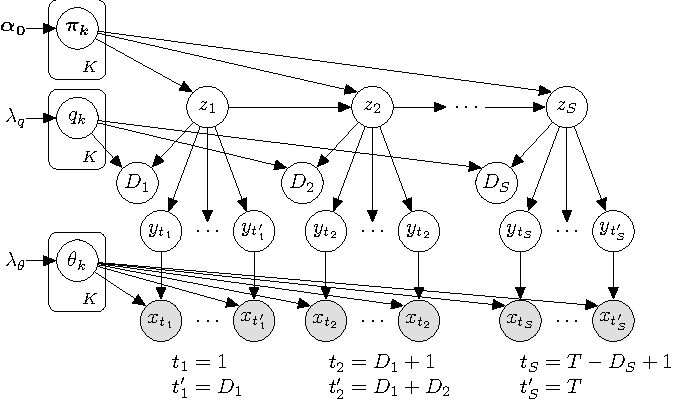
\includegraphics[width=10cm]{fig/HSMM_graphical_model.pdf}
		\caption{Graphical model of HSMM.}
	\end{center}
\end{figure}

The probabilistic generative process of HMM is shown below.
\begin{eqnarray}
	\boldsymbol{\pi_0} &\sim& \Dir(\boldsymbol{\pi} | \boldsymbol{\alpha_0}) \\
	\boldsymbol{\pi_{k}} &\sim& \Dir(\boldsymbol{\pi} | \boldsymbol{\alpha_0}) \\
	\theta_k &\sim& p(\theta | \lambda_\theta) \\
	q_k &\sim& p(q | \lambda_q) \\
	z_1 &\sim& \Cat(z | \boldsymbol{\pi_0})\\
	z_s &\sim& \Cat(z | \boldsymbol{\pi_{z_{s-1}}})\\
	D_s &\sim& p(D | q_{z_s}) \\
	t_s &=& 1 + \sum_{s'=1}^{s-1}{D_{s'}} \\
	t'_s &=& \sum_{s'=1}^{s}{D_{s'}} \\
	&=& t_s + D_s - 1 \\
	y_{t_s:t'_s} &=& z_s \\
	x_t  &\sim& p(x | \theta_{y_t})\\
	\nonumber \\
	k &=& 1, 2, \ldots, K \\
	s &=& 1, 2, \ldots, S \\
	t &=& 1, \ldots, T
\end{eqnarray}
Here, $\Dir$ represents the Dirichlet distribution, $\Cat$ represents the categorical distribution.
And, you can use the any emission distribution $p(x | \theta_{t})$ and prior  distribution $p(\theta | \lambda_\theta)$.
For example, set $p(x | \theta_{t})$ to multivariate normal distribution and set $p(\theta | \lambda_\theta)$ to normal-inverse-Wishart distribution.

\section{Posterior distribution}
This section shows the posterior distributions.

\subsection{Posterior distribution of $z_s$ and $D_s$}
When sample the super-state sequence $z_{1:S}$ and the duration of super-states $D_{1:S}$, basically we use the blocked Gibbs sampling.
In this section, we shows the sampling algorithm using blocked Gibbs sampling.
\par
In the blocked Gibbs sampling of HSMM, the super-state sequence $z_{1:S}$ and   the duration of super-states $D_{1:S}$ are sampled by the conditional posterior distribution $p(z_{1:S} , D_{1:S}| x_{1:T}, \boldsymbol{\pi_{0:K}}, \theta_{1:K}, q_{1:K})$.
The distribution is little bit redundancy, so, we don't write the $\boldsymbol{\pi_{0:K}}$, $\theta_{1:K}$ and $q_{1:K}$ often in condition part.
Here, $p(z_{1:S} , D_{1:S}| x_{1:T}$ can be described as follows.

\begin{eqnarray}
	p(z_{1:S}, D_{1:S} | x_{1:T})
	&=&
	\prod_{s=1}^{S}{\left\{ p(z_s, D_s  |  z_{1:s-1}, D_{1:s-1}, x_{1:T}) \right\}}\\
	&=&
	\prod_{s=1}^{S}{\left\{ p(z_s |  z_{1:s-1}, D_{1:s-1}, x_{1:T}) p(D_s | z_{1:s}, D_{1:s-1}, x_{1:T})\right\}} \nonumber \\
\end{eqnarray}
And then, the term regarding sampling the $z_s$ is as follows.
\begin{eqnarray}
	p(z_s = i |  z_{1:s-1}, D_{1:s-1}, x_{1:T})
	&\proptoas{z_s}&
	p(x_{1:T} | z_{1:s-1}, z_s = i, D_{1:s-1}) p(z_s = i | z_{1:s-1}, D_{1:s-1}) \nonumber \\ \\
	&\proptoas{z_s}&
	p(x_{t_s:T} | z_s = i) p(z_s = i | z_{s-1}) \\
	&=&
	\beta_{t_s}^{*}(i) p(z_s = i | z_{s-1})
\end{eqnarray}
And, the term regarding sampling the $D_s$ is as follows.
\begin{eqnarray}
	p(D_s | z_{1:s-1}, z_s = i, D_{1:s-1}, x_{1:T})
	&=&
	p(D_s | z_s = i, x_{t_s:T}) \\
	&=&
	\frac{p(D_s, x_{t_s:T} | z_s = i)}{p(x_{t_s:T} | z_s = i)}\\
	&=&
	\frac{p(x_{t_s:t_s+d-1} | z_s = i, D_s = d) p(x_{t_s+d:T} | z_s = i) p(D_s = d| z_s = i)}{p(x_{t_s:T} | z_s = i)} \nonumber \\
	\\
	&=&
	\frac{p(x_{t_s:t'_s} | z_s = i, D_s = d) p(x_{t_{s+1}:T} | z_s = i) p(D_s = d| z_s = i)}{p(x_{t_s:T} | z_s = i)} \\
	&=&
	\frac{p(x_{t_s:t'_s} | z_s = i, D_s = d) \beta_{t_{s+1}}(i) p(D_s = d| z_s = i)}{\beta_{t_s}^{*}(i)}
\end{eqnarray}
Here, the $\beta_{t_s}(i)$ and $\beta_{t_s}^{*}$ are backward message in HSMM.
The definition of backward message is as follows.
Simply said, the backward message $\beta_{t_s}(i)$ is the probability about the $x_{t_s:T}$ was generated after if $i$-th super-state was beginning at $t_s$.
\begin{eqnarray}
	\beta_{t_s}(i)
	&\defeq&
	p(x_{t_s:T} | z_{s-1} = i) \\
	\beta_{t_s}^{*}(i)
	&\defeq&
	p(x_{t_s:T} | z_s = i) \\
	\beta_{T}(i)
	&\defeq&
	1
\end{eqnarray}
In addition, those are calculated as follows.
\begin{eqnarray}
	\beta_{t_s}(i)
	&\defeq&
	p(x_{t_s:T} | z_{s-1} = i) \\
	&=&
	\sum_{j}{p(x_{t_s:T}, z_s = j | z_{s-1} = i)} \\
	&=&
	\sum_{j}{p(x_{t_s:T} | z_s = j, z_{s-1} = i) p(z_s = j | z_{s-1} = i)} \\
	&=&
	\sum_{j}{p(x_{t_s:T} | z_s = j) p(z_s = j | z_{s-1} = i)} \\
	&=&
	\sum_{j}{\beta_{t_s}^{*}(j) p(z_s = j | z_{s-1} = i)}
\end{eqnarray}
\begin{eqnarray}
	\beta_{t_s}^{*}(i)
	&\defeq&
	p(x_{t_s:T} | z_s = i) \\
	&=&
	\sum_{d=1}^{T-t_s}{p(x_{t_s:T}, D_s = d | z_s = i)} \\
	&=&
	\sum_{d=1}^{T-t_s}{p(x_{t_s:T} | z_s = i, D_s = d) p(D_s = d  | z_s = i)} \\
	&=&
	\sum_{d=1}^{T-t_s}{p(x_{t_s:t_s+d-1} | z_s = i, D_s = d) p(x_{t_s+d:T} | z_s = i, D_s = d) p(D_s = d  | z_s = i)} \nonumber \\ \\
	&=&
	\sum_{d=1}^{T-t_s}{p(x_{t_s:t'_s} | z_s = i, D_s = d) p(x_{t_{s+1}:T} | z_s = i) p(D_s = d  | z_s = i)} \\
	&=&
	\sum_{d=1}^{T-t_s}{p(x_{t_s:t'_s} | z_s = i, D_s = d) \beta_{t_{s+1}}(i) p(D_s = d  | z_s = i)}\\
t'_s &=& t_s + d - 1 \\
t_{s+1} &=& t_s + d
\end{eqnarray}

Summarize, the formulas about backward message are as follows.
\begin{eqnarray}
	\beta_{t_s}(i)
	&\defeq&
	p(x_{t_s:T} | z_{s-1} = i) \\
	\beta_{t_s}^{*}(i)
	&\defeq&
	p(x_{t_s:T} | z_s = i) \\
	\beta_{T}(i)
	&\defeq&
	1 \\
	\nonumber \\
	\beta_{t_s}(i)
	&=&
	\sum_{j}{\beta_{t_s}^{*}(j) p(z_s = j | z_{s-1} = i)} \\
	\beta_{t_s}^{*}(i)
	&=&
	\sum_{d=1}^{T-t_s}{p(x_{t_s:t'_s} | z_s = i, D_s = d) \beta_{t_{s+1}}(i) p(D_s = d  | z_s = i)} \\
	\nonumber \\
	t'_s &=& t_s + d - 1 \\
	t_{s+1} &=& t_s + d
\end{eqnarray}

\end{document}
